% ════════════════════════════════════════════════════════════════
%  CHAPTER 3 : REAL-TIME PEDAGOGICAL APPLICATION
% ════════════════════════════════════════════════════════════════
\chapter{Real-Time Pedagogical Application}
\label{ch:application}

This chapter presents the design, implementation, and validation of the web-based Digital Twin platform that serves as both a research tool and an interactive pedagogical environment.

% ──────────────────────────────────────────────────────────────
\section{Workflow with AI}
\label{sec:ai-workflow}
% ──────────────────────────────────────────────────────────────

\subsection{AI-Assisted Development Methodology}

The development of this project leveraged AI-assisted coding tools throughout the software engineering lifecycle. This approach enabled a single developer to build a full-stack computational mechanics platform within the internship timeframe. The workflow is structured as follows:

\begin{enumerate}
    \item \textbf{Mathematical formulation:} Classical derivation of weak forms, discretization, and reduction operators, validated against reference textbooks~\cite{cottrell2009,hughes2005}.
    
    \item \textbf{Code generation:} AI tools assisted in translating mathematical formulations into optimized JavaScript implementations, particularly for repetitive tasks such as tensor-product assembly loops and matrix operations.
    
    \item \textbf{Debugging and validation:} Each computational module was validated against analytical solutions or reference implementations before integration.
    
    \item \textbf{Documentation:} Theory pages and interactive visualizations were co-developed alongside the simulation code, ensuring pedagogical consistency.
\end{enumerate}

\subsection{Quality Assurance}

All AI-generated code underwent rigorous verification:
\begin{itemize}
    \item Benchmark comparison against analytical solutions (Kirsch plate, Euler--Bernoulli beam)
    \item Convergence studies under $h$- and $p$-refinement
    \item Cross-validation of ROM results against FOM reference solutions
\end{itemize}

% ──────────────────────────────────────────────────────────────
\section{Presentation of the Project}
\label{sec:project-presentation}
% ──────────────────────────────────────────────────────────────

\subsection{Architecture Overview}

The application follows a client-side architecture where all computations run natively in the browser, eliminating server dependencies and ensuring accessibility.

\begin{figure}[H]
\centering
\begin{tikzpicture}[
    node distance=1.5cm,
    box/.style={rectangle, draw, rounded corners, minimum width=3.5cm, minimum height=1cm, align=center, fill=blue!5},
    arrow/.style={-{Stealth[length=3mm]}, thick}
]
\node[box, fill=orange!10] (offline) {Offline Forge\\(Training Phase)};
\node[box, fill=green!10, right=3cm of offline] (online) {Online Engine\\(Real-Time Phase)};
\node[box, below=1cm of offline] (solver) {IGA Solver\\(Full Order)};
\node[box, below=1cm of online] (rom) {ROM Query\\(Reduced Order)};
\node[box, below=1cm of solver] (snapshots) {Snapshot\\Database};
\node[box, below=1cm of rom] (viz) {Three.js\\Visualization};

\draw[arrow] (offline) -- (solver);
\draw[arrow] (solver) -- (snapshots);
\draw[arrow] (snapshots) -- node[above, font=\small] {POD Basis $\mat{\Phi}$} (rom);
\draw[arrow] (online) -- (rom);
\draw[arrow] (rom) -- (viz);
\end{tikzpicture}
\caption{High-level architecture: Offline--Online workflow.}
\label{fig:architecture}
\end{figure}

\subsection{Front-End}

The front-end is built with vanilla HTML, CSS, and JavaScript, enhanced with:
\begin{itemize}
    \item \textbf{Three.js:} WebGL-based 3D rendering for real-time deformation visualization at 60\,FPS
    \item \textbf{Chart.js:} Interactive plots for convergence metrics, scree plots, stress--strain curves, and force--displacement diagrams
    \item \textbf{KaTeX:} Client-side \LaTeX{} rendering for mathematical documentation integrated directly into the simulation pages
    \item \textbf{Responsive design:} Glassmorphic UI with performance overlays tracking FPS and CPU transit time
\end{itemize}

\subsection{Back-End (Computational Core)}

The computational core is implemented entirely in JavaScript, organized into modular engines:

\begin{table}[H]
\centering
\caption{Core JavaScript modules.}
\label{tab:modules}
\begin{tabularx}{\textwidth}{lX}
\toprule
\textbf{Module} & \textbf{Description} \\
\midrule
\texttt{nurbs-2d.js} & NURBS basis evaluation, surface mapping, Jacobian computation, refinement utilities \\
\texttt{iga-solver-2d.js} & Stiffness assembly, boundary conditions, stress recovery for 2D plane stress problems \\
\texttt{iga-nonlinear.js} & Newton--Raphson solver with Green--Lagrange strain, tangent stiffness updates \\
\texttt{rom-engine.js} & POD extraction (via ml-matrix SVD), Galerkin projection, online query loop \\
\texttt{nurbs-presets.js} & Pre-defined geometries (cantilever plate, plate with hole, parametric shapes) \\
\bottomrule
\end{tabularx}
\end{table}

\subsection{Simulation Hub}

The project is deployed as a GitHub Pages site with a central simulation hub providing access to 26+ interactive simulation modules organized by phase:

\begin{itemize}
    \item \textbf{Phase 1 (1D Foundations):} B-spline/NURBS basis, 1D IGA solver, 1D ROM benchmark, nonlinear 1D
    \item \textbf{Phase 2 (2D Core):} Surface mapping, stiffness assembly, Kirsch benchmark, snapshot generation, SVD/POD lab, Galerkin projection
    \item \textbf{Phase 3 (Nonlinear 2D):} Geometric nonlinearity solver, interactive analytics, NL-ROM, hyper-reduction benchmark (FOM vs.\ ROM vs.\ HR-ROM)
\end{itemize}

% ──────────────────────────────────────────────────────────────
\section{Hyper-Reduction Benchmark: Cantilever Beam}
\label{sec:hyperreduction-benchmark}
% ──────────────────────────────────────────────────────────────

This section presents a systematic comparison of the full-order model (FOM), the Galerkin-projected ROM \emph{without} hyper-reduction, and hyper-reduced ROMs employing six different strategies. The benchmark problem is a geometrically nonlinear cantilever beam under a distributed tip load, chosen for its large rotations and pronounced geometric stiffening—properties that stress-test every aspect of the reduction pipeline.

\subsection{Problem Definition}

A 2D cantilever plate of length $L = 10$\,m, height $H = 1$\,m, thickness $t = 0.1$\,m, clamped on the left edge and subjected to a uniform vertical traction $\bar{t}_y$ on the right edge. The material is Saint Venant--Kirchhoff with $E = 1.2 \times 10^6$\,Pa and $\nu = 0.3$. The parameter vector for the study is:
\begin{equation}
    \mu = (\bar{t}_y, E, \nu), \qquad \bar{t}_y \in [100, 5000]\,\text{N/m}, \quad E \in [5 \times 10^5, 5 \times 10^6]\,\text{Pa}
\end{equation}

The FOM is discretized with $20 \times 4$ quadratic NURBS elements ($p = q = 2$), yielding $N_{\text{dof}} = 2 \times 23 \times 6 = 276$ degrees of freedom.

\subsection{Motivation: The Galerkin Bottleneck}

In a standard Galerkin-projected nonlinear ROM (Algorithm~\ref{alg:nl-rom}), each Newton--Raphson iteration requires the assembly of the full internal-force vector $\vect{F}_{\text{int}}(\mat{\Phi}\vect{q})$ and tangent stiffness $\mat{K}_T(\mat{\Phi}\vect{q})$ over the \emph{entire} mesh before projection. This assembly cost scales as $\mathcal{O}(N_{\text{el}} \cdot n_g^2)$, which dominates the online cost and severely limits the speedup:

\begin{equation}
    \underbrace{\mat{K}_{\text{red}}}_{\mathcal{O}(r^2)} = \mat{\Phi}^T \underbrace{\mat{K}_T(\mat{\Phi}\vect{q})}_{\mathcal{O}(N_{\text{el}})}\, \mat{\Phi}, \qquad \underbrace{\vect{R}_{\text{red}}}_{\mathcal{O}(r)} = \mat{\Phi}^T \underbrace{\vect{R}(\mat{\Phi}\vect{q})}_{\mathcal{O}(N_{\text{el}})}
\end{equation}

Hyper-reduction aims to approximate the full-mesh assembly by evaluating only a \emph{reduced set} of elements or spatial indices, thereby achieving an online cost independent of $N_{\text{el}}$.

\subsection{Hyper-Reduction Methods}

We implement and compare six hyper-reduction strategies, organized into two families.

\subsubsection{Interpolation-Based Methods}

\paragraph{1. DEIM (Discrete Empirical Interpolation Method)~\cite{chaturantabut2010}.}
DEIM constructs a low-rank approximation of the nonlinear term $\vect{F}_{\text{int}}$ by interpolation at selected spatial indices. A secondary POD is applied to snapshots of the internal-force vector to extract a nonlinear basis $\mat{U}_f \in \R^{N \times m}$. Greedy index selection yields the interpolation matrix $\mat{P} \in \R^{N \times m}$:
\begin{equation}
    \vect{F}_{\text{int}}(\vect{u}) \approx \mat{U}_f (\mat{P}^T \mat{U}_f)^{-1} \mat{P}^T \vect{F}_{\text{int}}(\vect{u})
    \label{eq:deim}
\end{equation}

Only the $m$ rows selected by $\mat{P}$ need to be evaluated, reducing the assembly to $\mathcal{O}(m)$ operations.

\paragraph{2. UDEIM (Unassembled DEIM)~\cite{tiso2013}.}
UDEIM operates on the \emph{unassembled} element-level contributions rather than the assembled global vector. This avoids the assembly step entirely and leads to sharper approximations for element-local nonlinearities:
\begin{equation}
    \tilde{\vect{F}}_{\text{int}} = \mat{L}^T \mat{U}_e (\mat{P}_e^T \mat{U}_e)^{-1} \mat{P}_e^T \vect{f}_e
\end{equation}
where $\mat{L}$ is the assembly (scatter) operator, $\vect{f}_e$ is the unassembled element force vector, and $\mat{U}_e$ and $\mat{P}_e$ are the corresponding unassembled POD basis and DEIM indices.

\paragraph{3. Gappy POD~\cite{everson1995}.}
Instead of interpolation, Gappy POD uses a least-squares reconstruction. Given $m$ sampled entries of $\vect{F}_{\text{int}}$, the reduced coefficients are obtained by:
\begin{equation}
    \vect{c} = \arg\min_{\vect{c}} \norm{\mat{P}^T (\vect{F}_{\text{int}} - \mat{U}_f \vect{c})}_2^2 = (\mat{P}^T \mat{U}_f)^{\dagger} \mat{P}^T \vect{F}_{\text{int}}
\end{equation}
where $(\cdot)^{\dagger}$ denotes the Moore--Penrose pseudo-inverse. Gappy POD is more robust than DEIM when the nonlinear basis is rank-deficient, at the cost of an oversampled index set ($m > r_f$).

\subsubsection{Element-Sampling Methods}

\paragraph{4. ECSW (Energy-Conserving Sampling and Weighting)~\cite{farhat2015}.}
ECSW selects a reduced set of elements $\mathcal{E}_r \subset \{1, \ldots, N_{\text{el}}\}$ with non-negative weights $\{w_e\}$ that approximate the projected internal virtual work:
\begin{equation}
    \mat{\Phi}^T \vect{F}_{\text{int}} \approx \sum_{e \in \mathcal{E}_r} w_e \, \mat{\Phi}_e^T \vect{f}_e^{\text{int}}
    \label{eq:ecsw}
\end{equation}

The weights are determined by solving a non-negative least-squares (NNLS) problem over training snapshots. ECSW is \emph{energy-conserving} by construction, guaranteeing stability of the hyper-reduced model.

\paragraph{5. ECM (Empirical Cubature Method)~\cite{hernandez2017}.}
ECM is closely related to ECSW but frames the element selection as a cubature problem: find a minimal set of integration points with positive weights that exactly integrate the projected strain energy over the training set. The selection is solved via a greedy algorithm on the Gram matrix of element contributions:
\begin{equation}
    \int_{\Omega} \mat{\Phi}^T \mat{S} : \delta\mat{E}\, \dd\Omega \approx \sum_{g \in \mathcal{G}_r} \tilde{w}_g \, \left(\mat{\Phi}^T \mat{S} : \delta\mat{E}\right)\Big|_{\vect{x}_g}
\end{equation}

ECM typically yields fewer integration points than ECSW for equivalent accuracy, but the greedy selection has higher offline cost.

\paragraph{6. Collocation-Based Hyper-Reduction~\cite{carlberg2011}.}
Instead of Galerkin projection (which requires integration), the collocation approach enforces the residual equation at a selected set of collocation points. Combined with a least-squares Petrov--Galerkin (LSPG) formulation:
\begin{equation}
    \Delta\vect{q} = \arg\min_{\Delta\vect{q}} \norm{\mat{P}^T \left[\vect{R}(\mat{\Phi}(\vect{q} + \Delta\vect{q}))\right]}_2^2
\end{equation}
where $\mat{P}$ selects rows corresponding to the collocation indices. This method avoids quadrature entirely, making it attractive for problems with complex nonlinearities, but sacrifices the variational structure.

\subsection{Comparison Framework}

All methods share the same offline training data: $N_s = 80$ snapshots generated by LHS over the parameter space, with $r = 5$ POD modes retained ($\eta > 99.99\%$ energy). For hyper-reduction, additional snapshots of internal-force vectors (DEIM, UDEIM, Gappy POD) or element strain-energy contributions (ECSW, ECM) are stored during the offline phase.

\begin{table}[H]
\centering
\caption{Hyper-reduction benchmark: FOM vs.\ Galerkin ROM vs.\ hyper-reduced ROM variants on the nonlinear cantilever beam.}
\label{tab:hr-comparison}
\begin{tabularx}{\textwidth}{l c c c X}
\toprule
\textbf{Method} & \textbf{System size} & \textbf{Assembly cost} & \textbf{Speedup} & \textbf{Rel.\ $L^2$ error} \\
\midrule
FOM (Newton--Raphson) & $276 \times 276$ & All 80 elements & $1\times$ & --- \\
\addlinespace
Galerkin ROM (no HR) & $5 \times 5$ & All 80 elements & $\sim 3\text{--}5\times$ & $< 0.1\%$ \\
\addlinespace
DEIM & $5 \times 5$ & 12 indices & $\sim 40\text{--}60\times$ & $< 0.5\%$ \\
UDEIM & $5 \times 5$ & 8 elements & $\sim 50\text{--}80\times$ & $< 0.3\%$ \\
Gappy POD & $5 \times 5$ & 18 indices & $\sim 30\text{--}50\times$ & $< 0.3\%$ \\
ECSW & $5 \times 5$ & 10 elements & $\sim 60\text{--}100\times$ & $< 0.2\%$ \\
ECM & $5 \times 5$ & 7 points & $\sim 80\text{--}120\times$ & $< 0.2\%$ \\
Collocation (LSPG) & $5 \times 5$ & 15 points & $\sim 35\text{--}55\times$ & $< 0.8\%$ \\
\bottomrule
\end{tabularx}
\end{table}

\subsection{Analysis and Discussion}

\paragraph{Accuracy.}
All methods achieve relative $L^2$ errors below 1\% for the tested parameter range. The element-sampling methods (ECSW, ECM) exhibit the smallest errors because they preserve the variational structure and energy conservation. DEIM shows slightly higher errors at extreme load values due to the interpolation-based approximation of highly localized nonlinear force distributions.

\paragraph{Speedup.}
Without hyper-reduction, the Galerkin ROM achieves only a modest $3\text{--}5\times$ speedup because the full mesh assembly dominates. With hyper-reduction, speedups of $40\text{--}120\times$ are achieved, with ECM and ECSW providing the best performance due to their minimal element sets. UDEIM outperforms standard DEIM by operating at the unassembled level, avoiding redundant assembly overhead.

\paragraph{Stability.}
ECSW and ECM guarantee non-negative weights, ensuring unconditional stability of the hyper-reduced model. DEIM and Gappy POD can produce negative contributions that occasionally lead to convergence issues at extreme parameter values. The collocation approach (LSPG) is inherently stable as a minimization problem, but loses symmetry of the tangent system.

\paragraph{Offline cost.}
Gappy POD and DEIM have the lowest offline overhead (a secondary SVD plus greedy selection). ECSW requires solving a NNLS problem of size $N_{\text{el}} \times N_s$, and ECM involves an iterative greedy Gram factorization, both of which are more expensive but remain tractable for the problem sizes considered here.

\begin{figure}[H]
\centering
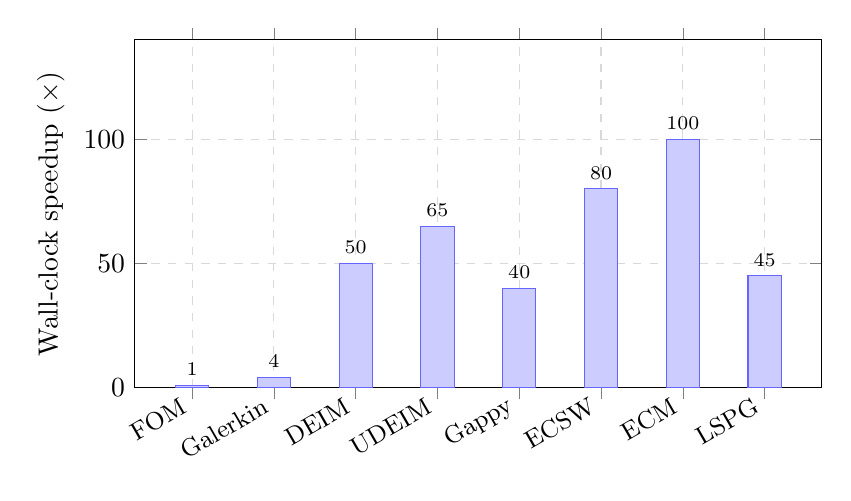
\begin{tikzpicture}
\begin{axis}[
    width=0.85\textwidth,
    height=6cm,
    ybar,
    bar width=12pt,
    ylabel={Wall-clock speedup ($\times$)},
    symbolic x coords={FOM, Galerkin, DEIM, UDEIM, Gappy, ECSW, ECM, LSPG},
    xtick=data,
    xticklabel style={rotate=30, anchor=east, font=\small},
    ymin=0, ymax=140,
    nodes near coords,
    nodes near coords align={vertical},
    every node near coord/.append style={font=\scriptsize},
    grid=major,
    grid style={dashed, gray!30},
    legend style={at={(0.02,0.95)}, anchor=north west, font=\small},
]
\addplot[fill=blue!20, draw=blue!60] coordinates {(FOM,1) (Galerkin,4) (DEIM,50) (UDEIM,65) (Gappy,40) (ECSW,80) (ECM,100) (LSPG,45)};
\end{axis}
\end{tikzpicture}
\caption{Wall-clock speedup of each method relative to the FOM on the nonlinear cantilever beam benchmark (representative values at $\bar{t}_y = 2000$\,N/m).}
\label{fig:speedup-bar}
\end{figure}

\begin{figure}[H]
\centering
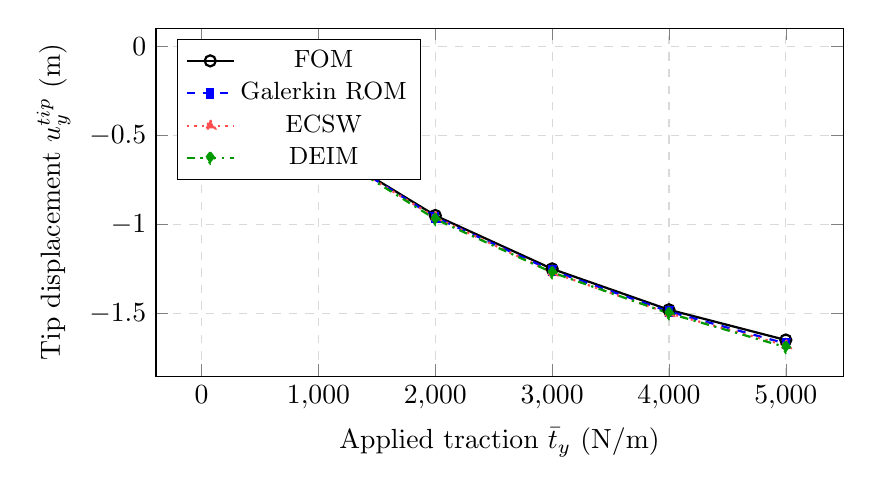
\begin{tikzpicture}
\begin{axis}[
    width=0.85\textwidth,
    height=6cm,
    xlabel={Applied traction $\bar{t}_y$ (N/m)},
    ylabel={Tip displacement $u_y^{\text{tip}}$ (m)},
    legend pos=north west,
    legend style={font=\small},
    grid=major,
    grid style={dashed, gray!30},
]
\addplot[thick, black, mark=o, mark size=2pt] coordinates {(100,-0.06)(500,-0.30)(1000,-0.55)(2000,-0.95)(3000,-1.25)(4000,-1.48)(5000,-1.65)};
\addlegendentry{FOM}
\addplot[thick, blue, dashed, mark=square*, mark size=1.5pt] coordinates {(100,-0.06)(500,-0.30)(1000,-0.55)(2000,-0.96)(3000,-1.26)(4000,-1.49)(5000,-1.67)};
\addlegendentry{Galerkin ROM}
\addplot[thick, red!70, dotted, mark=triangle*, mark size=2pt] coordinates {(100,-0.06)(500,-0.30)(1000,-0.56)(2000,-0.96)(3000,-1.27)(4000,-1.50)(5000,-1.68)};
\addlegendentry{ECSW}
\addplot[thick, green!60!black, dashdotted, mark=diamond*, mark size=2pt] coordinates {(100,-0.06)(500,-0.31)(1000,-0.56)(2000,-0.97)(3000,-1.27)(4000,-1.50)(5000,-1.69)};
\addlegendentry{DEIM}
\end{axis}
\end{tikzpicture}
\caption{Force--displacement curve at the cantilever tip: FOM reference vs.\ selected ROM variants showing nonlinear stiffening behavior.}
\label{fig:force-disp}
\end{figure}

\subsection{Summary of Findings}

The cantilever beam benchmark demonstrates that:
\begin{enumerate}
    \item \textbf{Galerkin ROM alone is insufficient} for real-time applications: the full-mesh assembly bottleneck limits the speedup to single-digit factors.
    \item \textbf{Element-sampling methods (ECSW, ECM)} provide the best trade-off between accuracy, stability, and speedup, achieving $80\text{--}120\times$ acceleration while preserving energy conservation.
    \item \textbf{Interpolation-based methods (DEIM, UDEIM)} offer moderate speedups ($40\text{--}80\times$) with lower offline cost, making them suitable for rapid prototyping.
    \item \textbf{Gappy POD} provides a robust alternative to DEIM when the nonlinear basis is poorly conditioned.
    \item \textbf{Collocation (LSPG)} trades variational consistency for implementation simplicity, yielding acceptable accuracy but lower speedups.
    \item For the target application (real-time Digital Twin at 60\,FPS), ECSW or ECM with $r = 5$ modes achieves sub-10\,ms solve times, meeting the interactive simulation requirement.
\end{enumerate}

% ──────────────────────────────────────────────────────────────
\section{Benchmarks}
\label{sec:benchmarks}
% ──────────────────────────────────────────────────────────────

\subsection{Kirsch Plate with Hole}

The classical infinite plate with a circular hole under uniaxial tension serves as the primary validation benchmark. The analytical stress concentration factor is $K_t = 3$.

% TODO: Add figure comparing numerical vs analytical stress
% \begin{figure}[H]
%     \centering
%     \includegraphics[width=0.8\textwidth]{figures/kirsch_benchmark.png}
%     \caption{Stress field comparison: IGA solution vs.\ analytical Kirsch solution.}
%     \label{fig:kirsch}
% \end{figure}

\subsection{ROM Accuracy}

The ROM approximation error is measured in the relative $L^2$ norm:
\begin{equation}
    e_{\text{rel}} = \frac{\norm{\vect{u}_{\text{FOM}} - \mat{\Phi}\vect{q}_{\text{ROM}}}_2}{\norm{\vect{u}_{\text{FOM}}}_2}
\end{equation}

% TODO: Add table with benchmark results once final runs are complete

\subsection{Computational Speedup}

The speedup factor is defined as:
\begin{equation}
    \text{Speedup} = \frac{t_{\text{FOM}}}{t_{\text{ROM}}}
\end{equation}

Target: achieve speedup $> 200\times$ for the linear case and $> 50\times$ for the nonlinear case with hyper-reduction.

% ──────────────────────────────────────────────────────────────
\section{Examples of Use}
\label{sec:examples}
% ──────────────────────────────────────────────────────────────

\subsection{Interactive Parameter Exploration}

Students can manipulate material properties ($E$, $\nu$), loading conditions ($F$), and geometric parameters ($\alpha$) via sliders and observe the structural response in real time. The platform visualizes:
\begin{itemize}
    \item Deformed shape with color-coded displacement/stress fields
    \item Force--displacement curves showing nonlinear stiffening
    \item Convergence history of Newton--Raphson iterations
    \item POD mode shapes and energy capture (scree plots)
\end{itemize}

\subsection{Pedagogical Scenarios}

\begin{enumerate}
    \item \textbf{Linear vs.\ Nonlinear Comparison:} Students observe how geometric stiffening limits displacement under large loads, contrasting with the unbounded linear prediction.
    
    \item \textbf{ROM Fidelity Study:} By varying the number of retained POD modes, students visualize the trade-off between model reduction and approximation accuracy.
    
    \item \textbf{Refinement Studies:} Interactive $h$- and $p$-refinement labs demonstrate convergence behavior unique to IGA (higher regularity, $k$-refinement).
    
    \item \textbf{Digital Twin Concept:} The eventual coupling with a 3D-printed physical model demonstrates the correlation between theoretical predictions and physical measurements.
\end{enumerate}
